\documentclass[12pt]{article}
\usepackage{color}
\usepackage{amsmath,amssymb}
\usepackage{fancyhdr}
\usepackage{graphicx}
\usepackage{listings}
\usepackage{lineno}
\graphicspath{ {../results/} }

\title{Autocorrelation in Weather}
\author{Victoria Blanchard}
\date{24th October 2019}


\begin{document}
    \maketitle

    \section{Correlate consecutive years}
        A Pearson's test was computed to asses the relationship between recorded temperatures over consecutive years. 

        There was a positive correlation between temperature and time (r = 0.326, n = 99, p < 0.01). 

        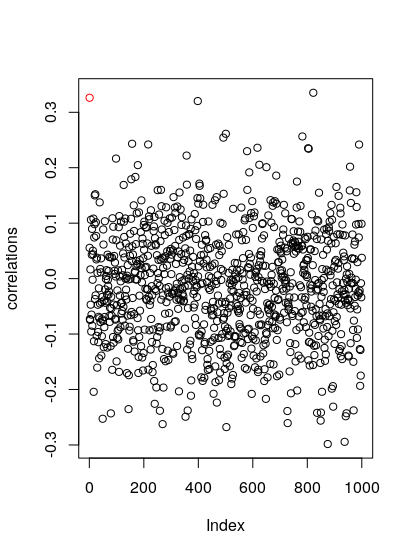
\includegraphics{Correlates.png}

        \verb+\lstinputlisting{simple.R}

    \section{Correlate randomly generated temperature data over consecutive years}
        A Pearson's test was computed to asses the relationship between random temperatures over inputted into dummy consecutive years. 

        Correlation values for random temperatures were almost always lower than the correlation value for the recorded data. This means that the probability that the data set was randomly generated is <0.01. 

        \includegraphics{./Correlates/}

\end{document}